\section{EINLEITUNG}\label{ch:einleitung}

OTH-Wiki ist eine Web-Anwendung, welche relevante Informationen für Studenten bereits stellt. \\ 
Nutzer der Seite, sehen dabei nur die Single-Page-Applikation, welche mittels Angular erstellt wurde.
Diese wird mittels eines Nginx-Servers ausgeliefert, welcher sich in einem Docker-Container befindet.
Um immer aktuelle Inhalte anzuzeigen, wird mittels einem Backend kommuniziert, welches mittels Python und FastAPI Informationen bereitstellt, und in einer MongoDB Datenbank sichert.
\begin{figure}[!htb]
    \centering
    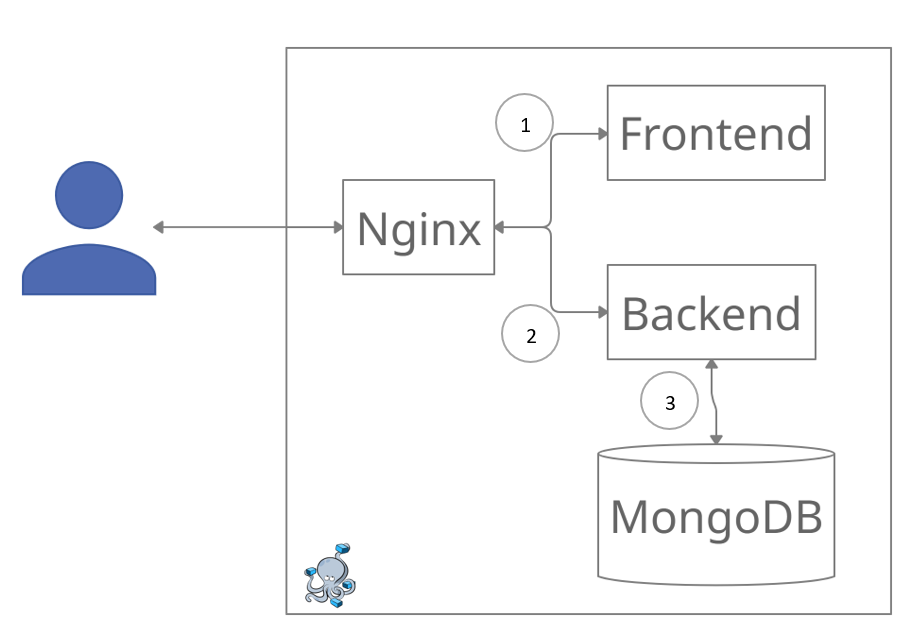
\includegraphics[width=7cm]{abbildungen/overview_architektur.PNG}
    \caption{Übersicht Architektur}
    \label{fig:arch}
\end{figure} 